\documentclass[aps,pra,reprint,superscriptaddress,longbibliography]{revtex4-2}

\usepackage[T1]{fontenc}
\usepackage{amsmath,amssymb,amsthm}
\usepackage{microtype}
\usepackage{graphicx}
\usepackage[colorlinks=true,linkcolor=blue,citecolor=blue,urlcolor=blue]{hyperref}
\graphicspath{{assets/}}

\newtheorem{theorem}{Theorem}
\newcommand{\dd}{\mathrm{d}}
\newcommand{\nvec}{\mathbf n}
\newcommand{\rvec}{\mathbf r}
\newcommand{\vvec}{\mathbf v}
\newcommand{\ez}{\mathbf e_z}
\newcommand{\sigmavec}{\boldsymbol\sigma}

% 两种语言版本共用英文图注。
\newcommand{\shortcorpsecaption}{Short-CORPSE attaining the robust $\pi$-gate time.
(a) The saturated control segments have durations
$(\pi/3,5\pi/3,\pi/3)/\Omega$, with $u_y=0$.
(b) The planar error curve consists of three unit-radius circular arcs
in dimensionless coordinates $\Omega\mathbf r$. It returns to its
starting point with opposite initial and final tangents. Colors identify
the same control segments in both panels.}


\begin{document}

\title{Exact time limit for first-order detuning-robust qubit
\texorpdfstring{$\pi$}{pi} gates}
\author{Tingyu Zhang}
\email{23300190021@m.fudan.edu.cn}
\affiliation{Department of Physics, Fudan University, Shanghai, China}
\author{Yan Cen}
\email[Corresponding author: ]{cenyan@fudan.edu.cn}
\affiliation{Department of Physics, Fudan University, Shanghai, China}

\begin{abstract}
We establish the exact minimum duration of a qubit $\pi$ gate that
cancels a constant detuning error to first order. For arbitrary measurable
transverse controls satisfying $u_x^2+u_y^2\le\Omega^2$, the minimum is
$7\pi/(3\Omega)$. The only controls attaining it are the known
short-CORPSE sequence and its overall negative, up to changes on sets of
measure zero. A second independently controlled transverse axis therefore
provides no time advantage for this task. The lower bound follows from a
sharp inequality valid in every dimension at least two: a unit-vector
curve with speed at most one, antipodal endpoints, and zero time average
has duration at least $7\pi/3$. Projection onto the curve's value at the
time midpoint gives the comparison and determines its equality cases.
The argument applies directly to measurable controls without requiring a
classification of extremal trajectories.
\end{abstract}
\maketitle

\section{Introduction}

A finite drive amplitude sets a time cost for suppressing systematic
errors during a quantum gate. Independent amplitude and phase control
enlarge the available pulse shapes, raising the question of whether this
freedom can reduce that cost. We address this question for a full qubit
$\pi$ gate with first-order robustness against static detuning, under a
joint amplitude bound on two transverse controls.

The short-CORPSE sequence has duration $7\pi/(3\Omega)$ and is optimal
within a symmetric family of three elementary pulses~\cite{kukita2022}.
Related planar geometric
constructions were developed for a single control
axis~\cite{zeng2018}. With two independent transverse controls, the
time-optimality of short-CORPSE has remained a separate question:
Pontryagin analysis identifies it as a candidate~\cite{kukita2024}, and
numerical optimization gives first-order robust $X$-gate durations near
$2.33\pi/\Omega$~\cite{cao2024}.

The control problem is closely related to bounded-curvature paths. The planar
three-arc return with reversed tangent appears as a teardrop trajectory
in the controllability construction of Sigalotti and
Chitour~\cite[Remark~2.2]{sigalotti2006}. Kim and Cheong explicitly give
$7\pi/3$ as the shortest planar bounded-curvature path between coincident
positions with opposite directions~\cite[Fig.~7 and the case $d=0$]{kim2013}.
The corresponding spatial problem permits additional trajectories:
general three-dimensional shortest-path and reachability analyses
include nonplanar extremals~\cite{sussmann1995,bae2025,bae2026}; related
spatial branches also occur in the classification of
$\infty$-elastica~\cite{moser2022}.

Here we prove that short-CORPSE remains time optimal over the full class
of measurable two-axis controls. The key step is a comparison inequality
for spatial curves, which supplies the lower bound beyond the planar
problem. This Schur-type tangent comparison~\cite{sullivan2008} projects
onto the midpoint tangent and uses the antipodal endpoints to constrain
both halves of the curve. Equality forces the curve into a single plane
and, with the full gate condition, fixes the control to short-CORPSE or
its overall negative.

\section{Control model and main result}
\label{sec:model}

We set $\hbar=1$ and take Pauli matrices with eigenvalues $\pm1$. The
propagator obeys
\begin{equation}
 \begin{aligned}
 \dot U_\delta(t)&=-\frac{i}{2}
 \bigl[u_x(t)\sigma_x+u_y(t)\sigma_y+\delta\sigma_z\bigr]U_\delta(t),
 \\
 U_\delta(0)&=I.
 \end{aligned}
 \label{eq:dynamics}
\end{equation}
Here $\delta$ is an unknown constant and the real controls are
measurable, independent of $\delta$, and satisfy the amplitude bound
\begin{equation}
 u_x(t)^2+u_y(t)^2\le\Omega^2
 \quad\text{for almost every }t,
 \label{eq:disk}
\end{equation}
where $\Omega>0$ is fixed. There is no independent longitudinal control.
A change of control
phase changes the subsequent transverse drive; it does not apply an
additional instantaneous gate. The admissible class includes reduced
amplitudes, zero-control intervals, and arbitrary phase changes.

Write $R_x(\theta)=\exp(-i\theta\sigma_x/2)$. Let $T_*$ be the
infimum of all durations $T>0$ for which an admissible control satisfies
\begin{equation}
 \begin{aligned}
 U_0(T)&=\pm R_x(\pi),\\
 \left.\partial_\delta U_\delta(T)\right|_{\delta=0}&=0.
 \end{aligned}
 \label{eq:target}
\end{equation}
The sign ignores an overall phase. The derivative condition is an
operator identity, so robustness holds for every input state.

\begin{theorem}[Exact robust gate time]
\label{thm:gate}
For the control class~\eqref{eq:disk} and target~\eqref{eq:target},
\begin{equation}
 \boxed{T_* = \frac{7\pi}{3\Omega}.}
 \label{eq:main}
\end{equation}
Apart from changes on sets of measure zero, the only minimizing controls
have $u_y=0$ and $u_x=\pm\Omega q(\Omega t)$, where $q$ has three
successive constant segments of values $+1,-1,+1$ and dimensionless
durations $\pi/3,5\pi/3,\pi/3$.
\end{theorem}

Thus the second transverse axis does not shorten this robust gate.
The lower bound applies to the full measurable control class;
planarity and the three-segment structure follow from equality.

\subsection{The toggling-frame error curve}

To obtain the lower bound, introduce the toggling-frame noise direction
and its integral:
\begin{equation}
 \begin{aligned}
 \nvec(t)\cdot\sigmavec&=U_0(t)^\dagger\sigma_zU_0(t),\\
 \rvec(t)&=\int_0^t\nvec(s)\,\dd s.
 \end{aligned}
 \label{eq:curve}
\end{equation}
This is the error-curve representation used in geometric robust
control~\cite{zeng2018,piliouras2026}. The identities needed here follow
directly from~\eqref{eq:dynamics}. Differentiation with respect to the
constant parameter $\delta$ gives the variation-of-constants formula
\begin{equation}
 \begin{aligned}
 \left.\partial_\delta U_\delta(T)\right|_0
 &=-\frac{i}{2}U_0(T)
 \int_0^T U_0(t)^\dagger\sigma_zU_0(t)\,\dd t
 \\
 &=-\frac{i}{2}U_0(T)\,\rvec(T)\cdot\sigmavec.
 \end{aligned}
 \label{eq:variation}
\end{equation}
Hence first-order detuning cancellation is equivalent to
$\rvec(T)=0$.

Unitary conjugation preserves the Pauli inner product, so $|\nvec|=1$.
Define the orthonormal vectors $\mathbf a,\mathbf b,\nvec$ by conjugating
$\sigma_x,\sigma_y,\sigma_z$, respectively. The commutator in the
derivative of~\eqref{eq:curve} yields
\begin{equation}
 \begin{aligned}
 \dot{\nvec}&=u_x\mathbf b-u_y\mathbf a,\\
 |\dot{\nvec}|&=\sqrt{u_x^2+u_y^2}\le\Omega
 \quad\text{a.e.}
 \end{aligned}
 \label{eq:speed}
\end{equation}
The endpoint gate imposes
\begin{equation}
 \nvec(0)=\ez,
 \qquad
 \nvec(T)=-\ez,
 \label{eq:antipodes}
\end{equation}
because $R_x(\pi)^\dagger\sigma_zR_x(\pi)=-\sigma_z$.
For bounded measurable controls, $U_0$ and $\nvec$ are Lipschitz and
$\rvec\in W^{2,\infty}$; all differential identities above hold almost
everywhere.

Rescaling time by $s=\Omega t$ thus produces an absolutely continuous
unit-vector curve of duration $L=\Omega T$, speed at most one,
antipodal endpoints, and zero integral. The following theorem proves
$L\ge7\pi/3$. The argument uses this forward map from controls to
curves; a direct calculation in Sec.~\ref{sec:attainment} establishes
attainment in the gate model.

\section{A sharp midpoint comparison}
\label{sec:midpoint}

\begin{theorem}[Antipodal zero-mean spherical curves]
\label{thm:sphere}
Let $d\ge2$ and let $\nvec:[0,L]\to S^{d-1}$ be absolutely continuous,
where $L>0$. Suppose that
\begin{equation}
 \begin{gathered}
 |\nvec'(t)|\le1\quad\text{a.e.},\qquad
 \nvec(L)=-\nvec(0),\\
 \int_0^L\nvec(t)\,\dd t=0.
 \end{gathered}
 \label{eq:spherical-assumptions}
\end{equation}
Then $L\ge7\pi/3$. The constant is sharp.
\end{theorem}

\begin{proof}
Set $c=L/2$ and $\vvec=\nvec(c)$. Spherical distance is bounded by
curve length, so
\begin{equation}
 d_S(\nvec(s),\nvec(t))\le|t-s|.
 \label{eq:lipschitz-sphere}
\end{equation}
If $c<\pi$, this gives
\begin{equation}
 \begin{aligned}
 \vvec\cdot\int_0^{2c}\nvec(t)\,\dd t
 &\ge\int_0^{2c}\cos|t-c|\,\dd t\\
 &=2\sin c>0,
 \end{aligned}
 \label{eq:first-lower}
\end{equation}
contrary to the zero integral. We may therefore assume $c\ge\pi$.

Let $\alpha=d_S(\vvec,\nvec(0))$. The antipodal endpoint has distance
$\pi-\alpha$ from $\vvec$. Consider either half of the curve, oriented
from its endpoint towards $\vvec$, and denote it by
$\mathbf m:[0,c]\to S^{d-1}$. If
$\beta=d_S(\vvec,\mathbf m(0))$, the triangle inequality and
\eqref{eq:lipschitz-sphere} imply
\begin{equation}
 d_S(\vvec,\mathbf m(t))
 \le\min\{\beta+t,c-t,\pi\}.
 \label{eq:envelope}
\end{equation}
Since cosine is decreasing on $[0,\pi]$,
\begin{equation}
 \int_0^c\vvec\cdot\mathbf m(t)\,\dd t
 \ge A(c,\beta),
 \label{eq:half-bound}
\end{equation}
where direct integration gives
\begin{align}
 A(c,\beta)
 &:=\int_0^c
 \cos\bigl(\min\{\beta+t,c-t,\pi\}\bigr)\,\dd t
 \nonumber\\
 &=\begin{cases}
 2\sin\bigl((c+\beta)/2\bigr)-\sin\beta,
       &c+\beta\le2\pi,\\[1mm]
 2\pi-c-\beta-\sin\beta,
       &c+\beta\ge2\pi.
 \end{cases}
 \label{eq:A}
\end{align}
Indeed, in the first case the two affine bounds meet at
$t=(c-\beta)/2$. In the second, their minimum is capped at $\pi$ for
an interval of length $c+\beta-2\pi$. The formula applies because
$0\le\beta\le\pi\le c$. Applied to both halves,
\eqref{eq:half-bound} yields
\begin{equation}
 0\ge A(c,\alpha)+A(c,\pi-\alpha).
 \label{eq:necessary}
\end{equation}

We evaluate the right-hand side at $c_*=7\pi/6$. Write
\begin{equation}
 B(\alpha)=A(c_*,\alpha)+A(c_*,\pi-\alpha).
 \label{eq:B}
\end{equation}
By symmetry, it suffices to consider $0\le\alpha\le\pi/2$.
If $\pi/6\le\alpha\le\pi/2$, both terms use the first branch
of~\eqref{eq:A}. With
$x=\cos(\alpha/2-\pi/4)\in[\sqrt3/2,1]$, one obtains
\begin{align}
 B(\alpha)
 &=4\sin(5\pi/6)x-2\sin\alpha\nonumber\\
 &=2x-2(2x^2-1)
 =2(1-x)(2x+1)\ge0.
 \label{eq:B-middle}
\end{align}
If $0\le\alpha\le\pi/6$, the second term in~\eqref{eq:B}
uses the capped branch, so
\begin{equation}
 \begin{aligned}
 B(\alpha)={}&2\sin(7\pi/12+\alpha/2)\\
 &+\alpha-\pi/6-2\sin\alpha.
 \end{aligned}
 \label{eq:B-edge}
\end{equation}
Its derivative is strictly negative on this interval:
\begin{equation}
 \begin{aligned}
 B'(\alpha)&=\cos(7\pi/12+\alpha/2)+1-2\cos\alpha\\
 &<0.
 \end{aligned}
 \label{eq:B-edge-derivative}
\end{equation}
Consequently $B(\alpha)\ge B(\pi/6)=\sqrt3-1>0$.
Together with symmetry, these calculations show
\begin{equation}
 \begin{gathered}
 B(\alpha)\ge0\quad(0\le\alpha\le\pi),\\
 B(\alpha)=0\ \Longleftrightarrow\ \alpha=\pi/2.
 \end{gathered}
 \label{eq:B-positive}
\end{equation}

Finally, fix $\beta\in[0,\pi]$. For $\pi<c\le c_*$,
the derivative of $A$ with respect to $c$ is either
$\cos((c+\beta)/2)<0$ in the uncapped branch or $-1$ in the
capped branch. These derivatives agree at the branch boundary.
Thus, whenever $\pi\le c<c_*$,
\begin{equation}
 A(c,\beta)>A(c_*,\beta).
 \label{eq:strict-monotonicity}
\end{equation}
Equations~\eqref{eq:necessary}, \eqref{eq:B-positive}, and
\eqref{eq:strict-monotonicity} would then give
\begin{equation}
 0\ge A(c,\alpha)+A(c,\pi-\alpha)>B(\alpha)\ge0,
\end{equation}
a contradiction. Hence $c\ge c_*$, or $L\ge7\pi/3$.
The planar curve constructed in Sec.~\ref{sec:attainment} attains
equality and embeds into every $S^{d-1}$ with $d\ge2$.
\end{proof}

The same result can be stated directly for spatial curves. If
$\rvec\in W^{2,\infty}([0,L];\mathbb R^d)$ has
$|\rvec'|=1$, $|\rvec''|\le1$ almost everywhere,
$\rvec(L)=\rvec(0)$, and $\rvec'(L)=-\rvec'(0)$, then its length is
at least $7\pi/3$. Taking $\nvec=\rvec'$ proves this assertion.
Self-intersections and curvature discontinuities are allowed.

\section{Attainment and all equality cases}
\label{sec:attainment}

\begin{figure*}[t]
\centering
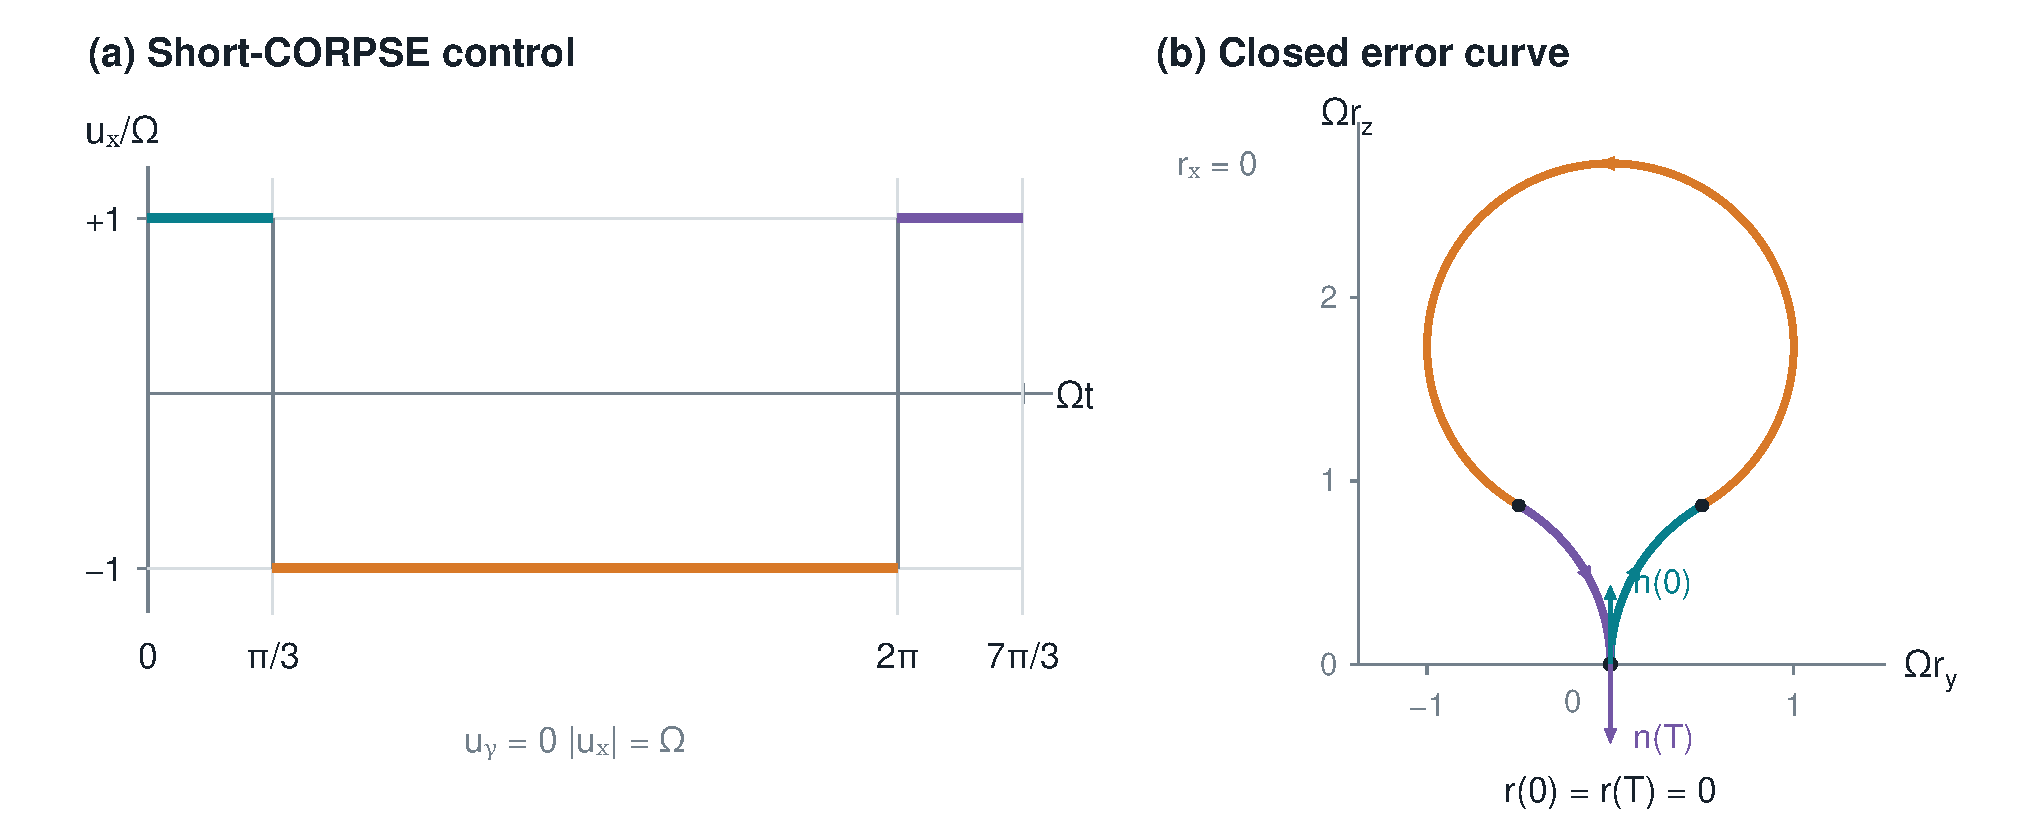
\includegraphics[width=0.92\textwidth]{short_corpse_geometry.pdf}
\caption{\shortcorpsecaption}
\label{fig:attainment}
\end{figure*}

\subsection{The attaining pulse}

For completeness, we verify the known attaining pulse in the same
normalization as the lower bound; see Fig.~\ref{fig:attainment}.
Use dimensionless time $s=\Omega t$
and set $u_y=0$ and
\begin{equation}
 \frac{u_x}{\Omega}=q(s):=
 \begin{cases}
 +1,&0\le s<\pi/3,\\
 -1,&\pi/3\le s<2\pi,\\
 +1,&2\pi\le s\le7\pi/3.
 \end{cases}
 \label{eq:short-corpse}
\end{equation}
Let $\phi(s)$ be the accumulated signed rotation angle. At the three
successive segment endpoints it takes the values
$\pi/3$, $-4\pi/3$, and $-\pi$. Since all three Hamiltonians
commute,
\begin{equation}
 U_0(T)=R_x(-\pi)=-R_x(\pi).
 \label{eq:attaining-gate}
\end{equation}
Moreover,
\begin{equation}
 \nvec(s)=(0,\sin\phi(s),\cos\phi(s)).
 \label{eq:attaining-tangent}
\end{equation}
The $x$ component of its integral vanishes. For the other two,
integration on the three segments gives
\begin{align}
 i\int_0^{7\pi/3}e^{i\phi(s)}\,\dd s
 &=2e^{i\pi/3}-2e^{-i4\pi/3}
 \nonumber\\
 &\quad+e^{-i\pi}-1=0.
 \label{eq:attaining-error}
\end{align}
The real and imaginary parts therefore establish $\rvec(T)=0$,
and~\eqref{eq:variation} proves first-order gate robustness.
This supplies the upper bound matching Theorem~\ref{thm:sphere}.

The pulse also explains sharpness of the midpoint comparison. At
$c_*=7\pi/6$ its accumulated angle is $-\pi/2$, so the midpoint
tangent is $\vvec=-\mathbf e_y$, perpendicular to both endpoint
tangents. On either half of the curve, oriented from its endpoint
towards the midpoint, the spherical distance to $\vvec$ is exactly
\begin{equation}
 \begin{gathered}
 d_S(\vvec,\mathbf m(t))=\min\{\pi/2+t,c_*-t\},\\
 0\le t\le c_*.
 \end{gathered}
 \label{eq:saturating-envelope}
\end{equation}
Its projected integral is
$A(c_*,\pi/2)=2\sin(5\pi/6)-1=0$ on each half.
Thus the pulse attains both the pointwise distance comparison and its
integrated zero bound.

\subsection{Geometric rigidity and uniqueness of the control}
The comparison also determines all minimizers. Suppose that
$L=7\pi/3$. Equation~\eqref{eq:B-positive} forces $\alpha=\pi/2$.
The two continuous, nonnegative gaps in~\eqref{eq:half-bound} must
then vanish identically. Orient each half from the midpoint towards
its endpoint, calling it $\mathbf m:[0,c_*]\to S^{d-1}$. Its distance
from $\vvec$ is therefore
\begin{equation}
 f(s)=\min\{s,5\pi/3-s\},\qquad 0\le s\le c_*.
 \label{eq:rigidity-f}
\end{equation}
For $s>0$, write
\begin{equation}
 \mathbf m(s)=\cos f(s)\,\vvec+\sin f(s)\,\mathbf e(s),
\end{equation}
where $\mathbf e(s)\perp\vvec$ and $|\mathbf e(s)|=1$.
Because $0<f(s)\le5\pi/6<\pi$, the vector $\mathbf e$ is absolutely
continuous on every $[\varepsilon,c_*]$. Almost everywhere there,
\begin{equation}
 |\mathbf m'|^2=(f')^2+\sin^2 f\,|\mathbf e'|^2\le1.
 \label{eq:rigidity-speed}
\end{equation}
As $|f'|=1$ almost everywhere, $\mathbf e$ is constant. At the two
endpoints $f(c_*)=\pi/2$, so these constants are respectively
$\nvec(0)$ and $-\nvec(0)$. Thus both halves lie in the same great
circle, and the only equality curves are the three-arc trajectory
above, with arbitrary overall orientation.

For the gate problem this also fixes the controls. Given an equality
curve with midpoint tangent $\vvec\perp\ez$, let
$\mathbf a=\ez\times\vvec$. The explicit fixed-axis evolution
$U_a(t)=\exp[-i\phi(\Omega t)\mathbf a\cdot\sigmavec/2]$ generates
that curve, where $\phi$ is the accumulated signed angle of
pulse~\eqref{eq:short-corpse}.
If another admissible evolution $U_0$ generates the same $\nvec$,
then $W=U_0U_a^\dagger$ commutes with $\sigma_z$, hence is diagonal.
Its derivative satisfies
\begin{equation}
 \dot W=-iH_0W+iWH_a,
 \label{eq:lift-uniqueness}
\end{equation}
where both nominal Hamiltonians $H_0,H_a$ are off-diagonal in the
$\sigma_z$ basis. The right-hand side is off-diagonal, whereas
$\dot W$ is diagonal. Therefore $\dot W=0$ almost everywhere and
$W=I$. Finally, $U_a(T)=i\mathbf a\cdot\sigmavec$ equals
$\pm R_x(\pi)$ only when $\mathbf a=\pm\mathbf e_x$. Up to changes
on null sets, the only time-optimal controls are consequently
\eqref{eq:short-corpse} and its overall negative.
This completes the uniqueness assertion in Theorem~\ref{thm:gate}.

A Lean 4 formalization of the exact minimum time, attainment, and
classification of all minimizing controls accompanies the source files.



\section{Discussion}

The shortest error-free $\pi$ gate has duration $\pi/\Omega$:
the endpoint condition~\eqref{eq:antipodes} requires a spherical
distance $\pi$, and a constant drive at amplitude $\Omega$ attains
that time. First-order cancellation of static detuning increases the
exact minimum by a factor $7/3$. Geometrically, cancellation requires
the integrated noise direction to return to the origin. Its turn rate
is limited by the available drive, and the midpoint comparison
quantifies the additional time required to balance that integral.

Allowing a second transverse component enlarges the set of possible
noise-direction paths to spatial curves. Theorem~\ref{thm:sphere}
bounds this full class with the same constant achieved by a planar
three-arc trajectory. This is why independent phase control gives no
time advantage for the stated $\pi$-gate task. The proof includes
arbitrary switching and nonsaturated amplitudes through the single
almost-everywhere speed bound.

The spatial lower bound establishes the optimality of the known
$7\pi/3$ planar construction~\cite{kukita2022,sigalotti2006,kim2013}
over the full control disk. Its equality conditions explain why the
additional spatial freedom does not produce another minimizing control.
The special
antipodal endpoint identity is essential to the comparison. Other
target angles carry different endpoint information and, for full gate
synthesis, additional frame constraints. Determining their minimum
robust times requires a separate analysis.

The convex planar reference-arc hypothesis in classical Schur
comparison~\cite[Theorem~5.1]{sullivan2008} is not satisfied by this
three-arc return. Moser's sufficient global-optimality criterion for
$\infty$-elastica~\cite[Theorem~3]{moser2022}, in the unweighted case,
requires a nonzero
auxiliary function $g$ satisfying $0\le g\le-\boldsymbol\lambda\cdot\nvec$
for a constant vector $\boldsymbol\lambda$. Zero total displacement
would force $\int g=0$, excluding that criterion here. The midpoint
estimate supplies a comparison specifically adapted to antipodal
tangents and zero displacement.

\section{Conclusion}
\label{sec:conclusion}

Under the joint amplitude bound on arbitrary measurable transverse
controls, the exact minimum time for a first-order detuning-robust qubit
$\pi$ gate is $7\pi/(3\Omega)$. Only short-CORPSE and its overall
negative attain this time, with segment durations
$(\pi/3,5\pi/3,\pi/3)/\Omega$. The sharp midpoint comparison establishes
both the time limit and the equality structure while preserving the full
gate condition. Thus a second transverse control axis cannot reduce the
time cost of first-order static-detuning cancellation for this gate.

\begin{acknowledgments}
[ACKNOWLEDGMENTS AND FUNDING TO BE COMPLETED]
\end{acknowledgments}

\section*{Data and code availability}
[DATA AND CODE AVAILABILITY TO BE CONFIRMED]

\section*{Declarations}
[DECLARATIONS TO BE CONFIRMED]

% PRA 自动采用 apsrev4-2，并由 longbibliography 启用文献题名。
\bibliography{references}
\end{document}
